%SourceDoc ws-skript.tex
%
% c02-laplace.tex
%
% (c) 2006 Prof. Dr. Andreas M�ller
% $Id: c02-laplace.tex,v 1.13 2008/11/02 00:12:44 afm Exp $
%
\rhead{Laplace-Ereignisse}
\chapter{Wahrscheinlichkeit und Kombinatorik
\label{chapter-wahrscheinlichkeit-und-kombinatorik}}
In einigen der Beispiele haben wir intuitiv angenommen, dass
die m"oglichen
Elementarereignisse alle gleich wahrscheinlich sind. Ein unverf"alschter W"urfel
sollte jede Augenzahl mit der gleichen Wahrscheinlichkeit zeigen. Und beim
Roulette im Casino erwarten wir, dass die Kugel im Roulette-Rad mit der gleichen
Wahrscheinlichkeit in die einzelnen Zahlen landet. Somit lassen sich
Wahrscheinlichkeiten berechnen, indem die Zahl der m"oglichen Ausg"ange
gez"ahlt werden, also mit Hilfe von Kombinatorik.
Dieses Kapitel fasst weiter Beispiele zusammen, f"ur welche diese
speziellen Voraussetzungen zutreffen.

\section{Laplace-Ereignisse\label{section-laplace-ereignisse}}
Pierre Simon Laplace hat Wahrscheinlichkeitsbetrachtungen unter folgender
\index{Laplace-Ereignis}
\index{Laplace, Pierre Simon}
Annahme durchgef"uhrt:
\begin{annahme}In einem endlichen Wahrscheinlichkeitsraum $\Omega$ haben
alle Elementarereignisse die gleiche Wahrscheinlichkeit. Insbesondere
gilt
\[
P(A) = \frac{|A|}{|\Omega|}
\]
\end{annahme}
Unter dieser Voraussetzung l"auft das Bestimmen der Wahrscheinlichkeit
darauf hinaus, die Anzahl der m"oglichen F"alle zu z"ahlen, in denen
das Ereignis eintritt, Wahrscheinlichkeitsrechung ist somit eng verwandt
mit Kombinatorik.

\section{Erste Beispiele}
In diesem Abschnitt werden einige Bespiele von Wahrscheinlichkeitsr"aumen
und Wahrscheinlichkeiten beschrieben, die sich mit dem Ansatz von Laplace
erfolgreich behandeln lassen.

\subsection{M"unze werfen}
\index{Munze@{M\"unze, faire}}
Wirft man eine M"unze, kann sie nur auf einer von zwei Seiten landen,
die Elementarereignisse sind also $\Omega = \{\text{Kopf}, \text{Zahl}\}$.
Die mathematisch idealisierte M"unze ist so d"unn, dass sie nicht auf
der Kante stehen kann. Nach allgemeiner Erfahrung funktioniert f"ur
solche M"unzen der Ansatz von Laplace, d.h. $P(\text{Kopf}) = \frac12$
und $P(\text{Zahl})=\frac12$.

Selbstverst"andlich gibt es auch M"unzen, f"ur die die Laplace-Annahme
nicht funktioniert, gebogene M"unzen fallen zum Beispiel bevorzugt auf die
nach aussen gew"olbte Fl"ache.

\subsection{W"urfeln}
\index{Wurfel@{W\"urfel, fairer}}
W"urfel haben sechs Seiten, die gem"ass Laplace mit gleicher
Wahrscheinlichkeit obenliegen werden, die Wahrscheinlichkeit jedes
Resultates ist also gleich $P(i) = \frac12, i\in\{1,2,3,4,5,6\}$.
Wird eine Seite des W"urfels beschwert, f"allt er bevorzugt auf diese
Seite, und die Wahrscheinlichkeiten sind nicht mehr gleich.

\begin{figure}
\begin{center}
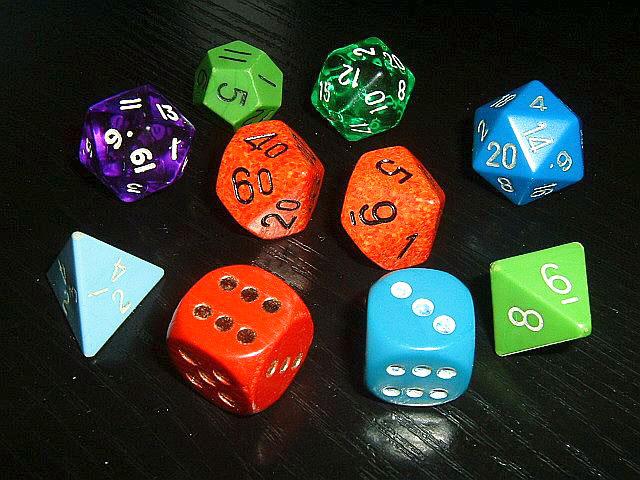
\includegraphics[width=0.8\hsize]{graphics/Wuerfel5}
\end{center}
\caption{Verschiedene Spielw"urfel\label{bild-spielwuerfel}}
\end{figure}
Man kann auch aus anderen geometrischen K"orpern ``W"urfel'' bauen, die
eine gr"ossere Zahl von Ausg"angen erm"oglichen. Ein Dodekaeder hat
zw"olf Seiten, ein Ikosaeder sogar deren 20, aber auch andere Formen
sind realisierbar, siehe Abbildung~\ref{bild-spielwuerfel}. Der Einfachheit
halber gehen wir im Folgenden immer von sechsseitigen W"urfeln aus.

Das werfen eines solchen W"urfels erzeugt die folgenden Elementarereignisse
oder Versuchsergebnisse:
\[
\Omega=\{1,2,3,4,5,6\}.
\]
Nach dem Laplace'schen Ansatz wird also jedem Elementarereignis die
Wahrscheinlichkeit $\frac16$ zugeschrieben. Damit lassen sich
Wahrscheinlichkeiten berechnen:
\begin{eqnarray*}
P(\text{``gerade Zahl''})=P(\{2,4,6\})&=&\frac36=0.5\\
P(\text{``durch 3 teilbar''})=P(\{3,6\})&=&\frac26=0.333\\
P(< 7)=P(\Omega)&=&\frac66=1\\
\end{eqnarray*}

\subsection{Zwei W"urfeln}
In verschiedenen Spielen wird mit zwei W"urfeln gespielt, wobei nur
deren Augensumme interessiert. Die Ereignisalgebra dazu wurde bereits
fr"uher vorgestellt, die Elementarereignisse sind Paare $(i,j)$ aus
den Augenzahlen der beiden W"urfel. Die Menge der Elementarereignisse
ist also
\begin{eqnarray*}
\Omega=&\{&\\
&&(1,1),(1,2),(1,3),(1,4),(1,5),(1,6),\\
&&(2,1),(2,2),(2,3),(2,4),(2,5),(2,6),\\
&&(3,1),(3,2),(3,3),(3,4),(3,5),(3,6),\\
&&(4,1),(4,2),(4,3),(4,4),(4,5),(4,6),\\
&&(5,1),(5,2),(5,3),(5,4),(5,5),(5,6),\\
&&(6,1),(6,2),(6,3),(6,4),(6,5),(6,6),\\
&\},&\\
\end{eqnarray*}
und $|\Omega|=36$. Wenn nur die Augensumme interessiert, dann will
man offensichtlich die Ereignisse
\begin{eqnarray*}
A_2&=&\{\Sigma=2\}=\{(1,1)\}\\
A_3&=&\{\Sigma=3\}=\{(1,2),(2,1)\}\\
A_4&=&\{\Sigma=4\}=\{(1,3),(2,2),(3,1)\}\\
&&\dots\\
A_{12}&=&\{\Sigma=12\}=\{(6,6)\}\\
\end{eqnarray*}
Diese Ereignisse sind einfach auszuz"ahlen, und damit kann man auch
die Wahrscheinlichkeiten bestimmen:
\begin{eqnarray*}
P(A_2)=P(A_{12})&=&\frac{1}{36}\\
P(A_3)=P(A_{11})&=&\frac{2}{36}\\
P(A_4)=P(A_{11})&=&\frac{3}{36}\\
P(A_5)=P(A_9)&=&\frac{4}{36}\\
P(A_6)=P(A_8)&=&\frac{5}{36}\\
P(A_7)&=&\frac{7}{36}\\
\end{eqnarray*}

\subsection{Die Reise nach Rom}
\index{Reise nach Rom}
Bei dem Kinder-Spiel die Reise nach Rom wird eine Anzahl $n$ St"uhle
im Kreis
aufgestellt, die um $1$ kleiner ist als die Anzahl der Teilnehmer.
Auf ein Signal versuchen alle Teilnehmer einen Sitzplatz zu
finden. In diesem Zusammenhang interesiert uns das Schicksal
desjenigen Teilnehmers nicht, der keinen Platz gefunden hat.
Stattdessen m"ochten wir die Wahrscheinlichkeit kennenlernen,
dass zwei Personen nebeneinander sitzen. Wir nehmen an, dass 
die Zuordnung von Sitzpl"atzen zu Teilnehmern zuf"allig erfolgt.
Elementarereignisse sind offenar die m"oglichen Anordnungen der
$n$ ``"uberlebenden'' Teilnehmer auf den $n$ St"uhlen. Das uns
interessierende Eregnis $A$ sind diejenigen Anordnungen, bei denen die
zwei Personen nebeneinander sitzen.

Die M"achtigkeit der Menge der Elementarereignisse $\Omega$ kann
wie folgt bestimmt werden. Der erste sitzende Teilnehmer hatte
$n$ St"uhle zur Auswahl. Zu jeder Wahl des ersten Teilnehmers bleiben
dem zweiten noch $n-1$ St"uhle, insgesamt kann man also die ersten
zwei Teilnehmer auf $n(n-1)$ Arten hinsetzen. Zu jeder Sitzordnung
der ersten zwei Kandidaten bleiben dem dritten Kandidaten $n-2$ Pl"atze
zur Wahl, also gibt es $n(n-1)(n-2)$ M"oglichkeiten, drei Kandidaten
auf $n$ Pl"atze zu setzen. So geht es weiter, bis zum
letzten Kandidaten, der keine wirkliche Wahl mehr hat, es gibt nur noch einen
freien Platz. Die Zahl der m"oglichen Sitzordnungen von $n$ Personen
auf $n$ St"uhlen ist also $n(n-1)(n-2)\dots 2\cdot 1$.

Zur Berechung der Wahrscheinlichkeit fehlt jetzt noch die Berechnung
von der Anzahl der Anordnungen, bei der die zwei Teilnehmer nebeneinander
sitzen. Offenbar gibt es $n$ M"oglichkeiten, wo der erste Teilnehmer
des Paars sitzen k"onnte, und je $2$ M"oglichkeiten, wo der zweite
Teilnehmer sitzen k"onnte, damit die zwei benachbart sind. Somit ist
die gesuchte Wahrscheinlichkeit
\[
P(A)=\frac{2n}{n!}.
\]

\subsection{Zuf"allige Auswahl}
Aus $n$ Elementen werden zuf"allig $k$ ausgew"ahlt. Wie gross ist die
Wahrscheinlichkeit, dass eine bestimmte Auswahl zustande kommt?

Elementarereignisse in diesem Problem sind offenbar die m"oglichen
Auswahlen, also $k$-elementige Teilmengen der $n$ Elemente. 
Dies sind die Kombinationen, also $\binom{n}k$. Die Wahrscheinlichkeit,
dass eine ganz bestimmte Auswahl zustande kommt, ist also 
\[
\frac1{\binom{n}k}
\]

%F"ur das erste gew"ahlte Element gibt es $n$ M"oglichkeiten,
%f"ur das zweite Element bleiben $n-1$ M"oglichkeiten, und so weiter
%bis zum $k$-ten Element f"ur welches $n-k+1$ M"oglichkeiten verbleiben.
%In diesem Prozess werden die $k!$ verschiedenen 
%Reihenfolgen einzeln gez"ahlt, obwohl sie zur selben ausgew"ahlten
%Teilmenge f"uhren.
%Die Zahl $k$-elementigen Teilmengen
%einer $n$-elementigen Menge ist daher
%\begin{align*}
%\binom{n}{k}
%&=
%\frac{n(n-1)\dots(n-k+1)}{k!}
%\\
%&=
%\frac{n(n-1)\dots(n-k+1)}{k!}
%\cdot
%\frac{(n-k)(n-k-1)\dots 1}{(n-k)(n-k-1)\dots 1}
%\\
%&=\frac{n!}{k!\,(n-k)!}
%\\
%&=\frac{n}{1}\cdot\frac{n-1}{2}\cdot \frac{n-2}{3}\dots\frac{2}{k-1}\cdot\frac1{k}
%\end{align*}
%Die letzte Form ist geeignet, den Binomialkoeffizienten
%auch f"ur grosse Zahlen $n$ zu berechnen, da sie sich vollst"andig
%in Ganzzahlarithmetik durchf"uhren l"asst. 
%
%Die Menge aller Teilmengen von l"asst sich unterteilen in die
%$k$-elementigen Teilmengen f"ur jeden Wert von $k$. Da es insgesamt
%$2^n$ Teilmengen einer $n$-elementigen Menge gibt, muss
%$$2^n=\sum_{k=0}^n\binom{n}{k}$$
%sein. Dies kann man nat"urlich auch aus der binomischen Formel
%gewinnen:
%$$(1+z)^n=\sum_{k=0}^n\binom{n}{k}z^k.$$
%Diese ist jedoch auch nur Ausdruck eines kombinatorischen
%Problems. Wegen
%$$(1+z)^n=(1+z)\dots(1+z)$$
%ist der Koeffizient von $z^k$ nichts anders als die Anzahl der
%M"oglichkeiten, aus dem Produkt auf der rechten Seite $k$ Faktoren
%auszuw"ahlen, in denen beim Ausmultiplizieren der Summand $z$ gew"ahlt wird.

\subsection{Meinungsumfrage}
\index{Meinungsumfrage}
Bei einer Meinungsumfrage versucht man im einfachsten Fall den Anteil
der Menschen an der Gesamtbev"olkerung vorherzusagen, die einer
Frage zustimmend oder ablehnend gegen"uberstehen. In dieser Form
ist das allerdings keine pr"azise Fragestellung.
Man k"onnte darunter zum Beispiel folgende verschiedenen Problem
verstehen:
\begin{enumerate}
\item Bestimme die Wahrscheinlichkeit, ein ``Ja'' als Antwort zu
erhalten, wenn man einen zuf"allig ausgew"ahlten Stimmberechtigten
nach seiner Meinung fragt.
\item Bestimme die Wahrscheinlichkeit, dass bei einer Abstimmung,
an der sich nur 60\%\ beteilign, die Abstimmungsfrage mit ``Ja''
beantwortet wird.
\end{enumerate}
Das sind allerdings zwei v"ollig verschiedene Fragen. In der ersten
Frage besteht das Experiment darin, eine Person auszuw"ahlen und nach
ihrer Meinung zu fragen. Die Menge der m"oglichen Elementarereignisse
ist also zun"achste die Menge aller Stimmberechtigten:
\[
\Omega=\{\text{``Stimmberechtigte''}\}.
\]
Die Antwort auf die Abstimmungsfrage ist ein Ja oder Nein, und sie
hat nichts mit Zufall zu tun, jedes mal, wenn man die Frage wieder
stellt, wird die Person gleich antworten. Also geht es hier um
die Anwendung einer Funktion $X$ auf die Person, die Funktion hat
Werte aus der Menge $\{0,1\}$:
\[
X\colon \Omega\to\{0,1\}.
\]
Mit dieser Ereignisalgebra kann man gem"ass Laplace zum Beispiel die
Frage beantworten,
wie gross die Wahrscheinlichkeit ist, dass ein Stimmberechtigter aus
dem Kanton Schwyz nach seiner Meinung gefragt wird.
Die Frage nach der Wahrscheinlichkeit f"ur ein ``Ja'' oder ``Nein''
steckt jedoch ausschliesslich im $X$ drin. Es ist n"amlich
\begin{eqnarray*}
P(\text{``Ja''})&=&P(\{\omega|X(\omega)=1\})\\
&=&\frac{|\{\omega|X(\omega)=1\}|}{|\Omega|}\\
&=&\frac{\text{Anzahl ``Ja''-Stimmer}}{\text{Anzahl Stimmberechtigte}}\\
\end{eqnarray*}
Offensichtlich kann man die Wahrscheinlichkeit nur ermitteln, wenn
man $X$ kennt.

Die zweite Frage beruht auf einer v"ollig anderen Ereignisalgebra. Hier
wird n"amlich nicht ein einzelner Stimmberechtigter gefragt, sonder
alle gleichzeitig, und es ist dabei auch nichts zuf"alliges, die
Leute haben ja eine eigene Meinung. Da aber das Meinungsforschungsinstitut
nicht alle Stimmberechtigten fragen kann (damit w"urde die Abstimmung
ja bereits durchgef"uhrt), befragt es nur eine {\bf zuf"allig} ausgew"ahlte
Gruppe. Der Zufall steckt also nicht in der Bev"olkerung, sondern in der
Auswahl der Repr"asentanten.

Die Frage lautet also genauer: wenn $M$ von $N$ Stimmberechtigte ``Ja''
stimmen, wie gross ist dann die Wahrscheinlichkeit, dass bei der Auswahl
von $n$ Stimmberechtigten deren $m$ ``Ja''-Sager sein werden?
Die Elementarereignisse sind in diesem Fall also Auswahlen von $n$
Stimmberechtigten, ein $\omega$ ist also eine Menge von Stimmberechtigen
mit genau $n$ Elementen:
\[
\omega=\{s_1,s_2,\dots,s_n\}
\]
$\Omega$ ist die Menge aller dieser Auswahlen. Zum Beispiel f"ur $n=3$:
\begin{eqnarray*}
\Omega=&\{&\\
&&\{\text{Heiri Muster}, \text{Peter Beispiel}, \text{Sara Sampler}\},\\
&&\{\text{Kora Werwohl}, \text{Anselm W"usstegern}, \text{Heiri Muster}\},\\
&&\{\text{Lara Croft}, \text{Paola}, \text{Udo J"urgens}\},\\
&&\dots\\
&\}&\\
\end{eqnarray*}
Es gibt $|\Omega|=\binom{N}{n}$ solche Teilmengen. Nun interessiert uns das
Ereignis, dass $m$ von diesen Stimmberechtigten ``Ja''-Sager sind, also
zu den $M$ ``Ja''-Sager geh"oren, die es gibt. Dieses Ereignis ist
die Menge
\[
A=\{\omega|\text{in $\omega$ hat es $m$ ``Ja''-Sager}\}.
\]
Offensichtlich kann
man eine solche Auswahl (ein $\omega)$
wie folgt erzeugen: zun"achst w"ahlt man $m$
``Ja''-Sager aus, und f"ullt dann mit $n-m$ zuf"allig ausgew"ahlten
``Nein''-Sagern aus. Es gibt $\binom{M}{m}$ M"oglichkeiten, $m$
``Ja''-Sager auszuw"ahlen, und $\binom{N-M}{n-m}$ M"oglichkeiten, $n-m$
``Nein''-Sager zu w"ahlen. F"ur jede ``Ja''-Sager-Auswahl gibt es
so viele ``Nein''-Sager-Auswahlen, also muss man die beiden Anzahlen
multiplizieren:
\[
|A|=\binom{M}{m}\binom{N-M}{n-m}.
\]
Nach Laplace ist also die Wahrscheinlichkeit, bei einer Stichprobe von
$n$ Stimmb"urgern $m$ ``Ja''-Sager zu finden:
\[
P(A)=\frac{\binom{M}{m}\binom{N-M}{n-m}}{\binom{N}{n}}.
\]
Das Problem, aus einer Menge von Individuen, die ein bestimmtes
Merkmal tragen, eine Stichprobe zu entnehmen, kommt in der Praxis immer
wieder vor. Daher lohnt es sich, ihm einen Namen zu geben:
\begin{definition}
\label{hypergeometrischeverteilung}
Die Wahrscheinlichkeit, bei einer $n$ Elemente umfassenden Stichprobe
aus einer $N$ Elemente grossen Gesamtheit, in der $M$ ein bestimmtes
Merkmal tragen, deren $m$ mit dem Merkmal zu finden ist
\[
h(m|N;M;n)=\frac{\binom{M}{m}\binom{N-M}{n-m}}{\binom{N}{n}}.
\]
$h$ heisst die ``hypergeometrische Verteilung''.
\end{definition}

\subsection{Geburtstagsproblem}
Wie gross ist die Wahrscheinlichkeit, dass unter $n$ Personen zwei
am gleichen Tag Geburtstag haben? Hierbei nimmt man an, dass
jeder Tag im Jahr etwa gleich h"aufig als Geburtstag
vorkommt\footnote{Dies ist
jedoch nicht ganz richtig, wie Geb"arabteilungen in Spit"alern
best"atigen k"onnen. Auch haben gr"osser Stromausf"alle h"aufig
einen Geburtenzuwachs ungef"ahr neun Monate sp"ater zur Folge.}.
Ein Elementarereignis muss also jeder der $n$ Personen ein
Geburtsdatum aus den $366$ m"oglichen zuweisen. Dies kann man so
formulieren:
\[
\omega=(d_1, d_2, d_3,\dots,d_n)
\]
Dabei ist $d_1$ das Geburtsdatum der ersten Person, $d_2$ das
Geburstdatum der zweiten Person, etc. Der einfachheit halber kann
man f"ur die $d_i$ einfach Zahlen zwischen 1 und 366 nehmen.

$\Omega$ besteht also aus allen m"oglichen Auswahlen von Geburtstagen
f"ur die $n$ Personen:
\begin{eqnarray*}
\Omega=&\{&\\
&&(1,1,1,\dots,1),\\
&&(2,1,1,\dots,1),\\
&&(3,1,1,\dots,1),\\
&&\dots\\
&&(365,1,1,\dots,1),\\
&&(366,1,1,\dots,1),\\
&&(1,2,1,\dots,1),\\
&&(2,2,1,\dots,1),\\
&&\dots\\
&&(366,366,366,\dots,366)\\
&\}&\\
\end{eqnarray*}
Man kann hier auch erkennen, dass $|\Omega|=366^n$ ist.

Gefragt ist nun das Ereignis
``zwei Personen haben am gleichen Tag Geburtstag''. 
Selbstverst"andlich d"urfen dabei auch alle am gleichen Tag
Geburstag haben, oder es darf zwei Paare geben, die jeweils
"ubereinstimmende Geburtstage haben. Es darf einfach nicht
sein, dass alle Geburtstage verschieden sind. Also ist eigentlich
gemeint:
\begin{eqnarray*}
A&=&\{\text{``zwei haben am gleichen Tag Geburstag''}\}\\
&=&\{\text{``nicht alle Geburtstage sind verschieden''}\}\\
&=&\overline{\{\text{``alle Geburstage sind verschieden''}\}}.\\
\end{eqnarray*}
In dieser letzten Form ist die Wahrscheinlichkeit einfacher zu
berechnen. Es gilt ja:
\begin{eqnarray*}
P(A)&=&P(\{\text{``zwei haben am gleichen Tag Geburstag''}\})\\
&=&1-P(\{\text{``alle Geburstage sind verschieden''}\})\\
\end{eqnarray*}
Die Anzahl der Geburtstagsverteilungen, bei denen alle Geburtstage
verschieden sind, ist einfach zu ermitteln: F"ur die erste Person
kann man $366$ Geburtstage ausw"ahlen, f"ur die zweite $365$, die
dritte $364$ etc. Insgesamt hat man
\[
366\cdot365\cdot364\dots(366-n+1)
\]
M"oglichkeiten. Also ist die Wahrscheinlichkeit, dass unter $n$
Personen zwei am gleichen Tag Geburtstag haben:
\[
P(A)=1-\frac{366\cdot365\cdot364\dots(366-n+1)}{366^n}.
\]
Man kann diese Wahrscheinlichkeiten mit einem kleinen Programm
ausrechnen, und findet die Resultate in
Tabelle~\ref{geburtstagswahrscheinlichkeit}.
\begin{table}
\begin{center}
\begin{tabular}{|c|c|c|c|c|c|c|c|}
\hline
$n$&$P$&$n$&$P$&$n$&$P$&$n$&$P$\\
\hline
1&0.0000
&11&0.1408
&21&0.4428
&31&0.7295\\
2&0.0027
&12&0.1666
&22&0.4748
&32&0.7524\\
3&0.0082
&13&0.1939
&23&0.5063
&33&0.7740\\
4&0.0163
&14&0.2226
&24&0.5373
&34&0.7944\\
5&0.0271
&15&0.2523
&25&0.5677
&35&0.8135\\
6&0.0404
&16&0.2829
&26&0.5972
&36&0.8313\\
7&0.0561
&17&0.3143
&27&0.6258
&37&0.8479\\
8&0.0741
&18&0.3461
&28&0.6534
&38&0.8633\\
9&0.0944
&19&0.3783
&29&0.6799
&39&0.8775\\
10&0.1166
&20&0.4106
&30&0.7053
&40&0.8905\\
\hline
\end{tabular}
\end{center}
\caption{Wahrscheinlichkeit daf"ur, dass unter $n$ Personen zwei
am gleichen Tag Geburtstag haben.\label{geburtstagswahrscheinlichkeit}}
\end{table}
Ab $n=23$ kann man also wetten, dass zwei Personen am gleichen Tag
Geburtstag haben.

\section{Berufswahlerhebung}
Dieses Beispiel soll illustrieren, dass auch bei Fragen, bei denen sehr
unterschiedliche Wahrscheinlichkeiten ausgegangen werden darf, im Hintergrund
ein Laplace-Prozess am Wirken ist.
Konkret geht es um die Frage nach der Wahrscheinlichkeit, dass ein 
zuf"allig ausgew"ahlter Lehrling einen bestimmten Beruf gew"ahlt hat.

Das Wahrscheinlichkeitsexperiment besteht darin, einen Lehrling
zuf"allig auszuw"ahlen. Hat man einen Lehrling ermittelt, kann man weiter
nachsehen, welchen Beruf er gew"ahlt hat. Die Menge der Elementarereignisse
ist also die Menge aller Lehrlinge. Die zuf"allige Auswahl eines Lehrlings
soll nat"urlich so geschehen, dass jedes Elementarereignis gleich
wahrscheinlich ist, d.h. die Wahrscheinlichkeit, dass ein ganz
bestimmter Lehrling gew"ahlt wird, ist
\[
p(\text{Heiri Muster})=\frac1{|\Omega|}=\frac1{|\{\text{Lehrlinge}\}|}.
\]

Die Bildungs"amter m"ochten nun aber "uber die Lehrlinge noch wesentlich mehr
wissen, hier eine Auswahl von m"oglichen Fragen:
\begin{enumerate}
\item Wie gross ist die Wahrscheinlichkeit, dass der Lehrling ein Mann/eine
Frau ist?
\item Wie gross ist die Wahrscheinlickeit, einen Elektromechaniker zu treffen?
\item Wie gross ist die Wahrscheinlichkeit daf"ur, eine Zahnarztgehilfin
zu treffen.
\end{enumerate}
Auf der Website der Deutschschweizerischen Berufsbildungs"amter-Konferenz
findet man umfangreiches Material zu diesen Fragen. Offensichtlich
sind alle Lehrlinge erfasst und gez"ahlt worden, und es ergaben sich
die auszugsweise in Tabelle \ref{berufswahldaten} dargestellten
Resultate.
\begin{table}
\begin{center}
\begin{tabular}{|l|r|r|r|}
\hline
Beruf&M"anner&Frauen&Total\\
\hline
Kaufm. Angestellte(r)&3944&6700&10644\\
Elektromonteur&2175&29&2204\\
Schreiner&1519&90&1609\\
Automechaniker&1309&37&1346\\
Koch&1296&589&1885\\
B"acker-Konditor&532&366&898\\
Handelsdiplomand&459&460&919\\
Verkaufslehre&1175&2985&4160\\
Floristin&10&430&440\\
Pharma-Assistentin&13&836&849\\
Zahnarztgehilfin&0&540&540\\
\hline
Insgesamt&37161&32192&69353\\
\hline
\end{tabular}
\end{center}
\caption{Berufswahldaten der Deutschschweizer Berufsbildungs"amter-Konferenz\label{berufswahldaten}}
\end{table}
Die Berufe der Lehrlinge und ihre Geschlechter definieren Teilmengen
der Lehrlinge, also Ereignisse. Die Menge aller B"acker $A_{\text{B"acker}}$
beinhaltet offensichtlich $898$ Elemente, die Wahrscheinlichkeit, dass ein
zuf"allig ausgew"ahlter Lehrling ein B"acker ist, ist also
\[
P(A_{\text{B"acker}})=\frac{|A_{\text{B"acker}}|}{|\Omega|}
=\frac{898}{69353}.
\]
Daneben gibt es auch die Ereignisse $B_{\text{Mann}}$ und $B_{\text{Frau}}$.
Die Wahrscheinlichkeit, dass ein zuf"allig gew"ahlter Lehrling ein Mann ist,
ist also $P(B_{\text{Mann}})=\frac{37161}{69353}$, f"ur die Frauen gilt
$P(B_{\text{Frau}})=1-P(B_{\text{Mann}})=\frac{32192}{69353}$.
Somit k"onnen weitere Ereignisse gebildet werden, zum Beispiel die
m"annlichen Handelsdiplomanden
$B_{\text{Mann}}\cap A_{\text{Handelsdiplomand}}$ und die
weiblichen Handelsdiplomanden
$B_{\text{Frau}}\cap A_{\text{Handelsdiplomand}}$.
Auch deren Wahrscheinlichkeit kann man berechnen:
\begin{eqnarray*}
P(A_{\text{Handelsdiplomand}})&=&\frac{919}{69353}\\
P(A_{\text{Handelsdiplomand}}\cap B_{\text{Mann}})&=&\frac{459}{69353}\\
P(A_{\text{Handelsdiplomand}}\cap B_{\text{Frau}})&=&\frac{460}{69353}\\
\end{eqnarray*}
Bei den Handelsdiplomanden scheint das Geschlecht auf die Berufswahl
wenig Einfluss zu haben. Insbesondere gilt n"aherungsweise
\[
P(A_{\text{Handelsdiplomand}}\cap B_{\text{Mann}})=P(A_{\text{Handelsdiplomand}})\cdot P(B_{\text{Mann}}).
\]
Wenn man aber die Elektromonteure und die Zahnarztgehilfinnen anschaut,
sieht es v"ollig anders aus.
\[
P(A_{\text{Zahnarztgehilfin}}\cap B_{\text{Mann}})=0\ne P(A_{\text{Zahnarztgehilfin}})\cdot P(B_{\text{Mann}}).
\]
Geschlecht und Beruf sind also nicht voneinander unabh"angig.
Die Wahrscheinlichkeit dass eine Frau Zahnarztgehilfin ist, ist viel
gr"osser, als dass ein Mann diesen Beruf gew"ahlt hat. Mit bedingten
Wahrscheinlichkeiten ausgedr"uckt:
\begin{eqnarray*}
P(A_{\text{Zahnarztgehilfin}}|B_{\text{Frau}})&=&\frac{|A_{\text{Zahnarztgehilfin}}\cap B_{\text{Frau}}|}{|B_{\text{Frau}}|}=1\\
P(A_{\text{Zahnarztgehilfin}}|B_{\text{Mann}})&=&\frac{|A_{\text{Zahnarztgehilfin}}\cap B_{\text{Mann}}|}{|B_{\text{Mann}}|}=0\\
\end{eqnarray*}

\section{Ziegen und Autos\label{ziegen:autos}}
Marylin vos Savant hat in einer Kolumne ein Gedankenexperiment vorgstellt.
In einer Quiz-Show muss der Kandidat eine von drei T"uren w"ahlen, wobei
sich hinter einer der T"uren ein Auto versteckt, hinter den anderen zweien
ein Ziege. Das Ziel des Spiels ist, das Auto zu gewinnen. Nach der Wahl
durch den Kandidaten "offnet der Quizmaster eine der T"uren, hinter der sich
eine Ziege befindet, nicht aber die T"ur, die der Kandidat gew"ahlt hat.
Der Kandidat hat jetzt nochmals die M"oglichkeit, die T"ur zu wechseln.
Welche Strategie soll er w"ahlen. Bei der ersten Auswahl bleiben, oder
wechseln?

Um die Frage zu beantworten berechnen wir die Gewinnwahrscheinlichkeit 
f"ur jede der Strategien. Zun"achst die ``Bleibe''-Strategie. Es ist die
Wahrscheinlichkeit f"ur einen Gewinn $P(G)$ auszurechnen. Hinter der zun"achst
gew"ahlten T"ur kann sich ein Auto (Ereignis $A$) befinden, oder eine Ziege
(Ereignis $Z$). Es ist nat"urlich $A\cap Z=\emptyset$ und $A\cup Z=\Omega$.
Also gilt
\begin{equation}
P(G)=P(G|A) P(A) + P(G|Z)P(Z).
\label{ziegenformel}
\end{equation}
Nat"urlich ist $P(A)=\frac13$ und $P(Z)=\frac23$.
$P(G|A)$ ist die Wahrscheinlichkeit mit der ``Bleibe''-Strategie zu
gewinnen, wenn hinter der zun"achst gew"ahlten T"ur ein Auto war: diese
ist nat"urlich 1. Ebenso verliert man mit sicherheit, wenn hinter der
T"ur eine Ziege war: $P(G|Z)=0$, also
\[
P(G)=P(G|A)P(A)+P(G|Z)P(Z)=1\cdot \frac13 + 0\cdot\frac 23=\frac13.
\]

F"ur die ``Wechsel''-Strategie gilt nat"urlich auch die Formel
\ref{ziegenformel}, aber die bedingten Wahrscheinlichkeiten sind verschieden.
Wenn man ein Auto gew"ahlt hatte, und wechselt, verliert man, also $P(G|A)=0$.
Hat man ein Ziege erwischt, und wechselt, bekommt man das Auto, denn die
zweite Ziege kann man ja nicht erwischen, deren T"ur hat der Quiz-Master
ge"offnet. Also ist $P(G|Z)=1$. Somit folgt jetzt
\[
P(G)=P(G|A)P(A)+P(G|Z)P(Z)=0\cdot\frac13+1\cdot\frac23=\frac23.
\]
Mit der Wechselstrategie ist also die Wahrscheinlichkeit, zu gewinnen,
doppelt so gross, wechseln lohnt sich also auf jeden Fall.

\section{Deal or no Deal}
Wir analysieren die folgende vereinfachte Form des Spiels Deal or no Deal.
Eine Anzahl $n$ von Koffern steht f"ur den Kandidaten zur Wahl.
Die Koffer enthalten viele kleine Preise, die wir als wertlos betrachten,
doch einer der Koffer enth"alt einen grossen Preis.
In jeder Runde w"ahlt der Kandidat einen Koffer. Der Moderator "offnet
dann einen wertlosen Koffer und gibt dem Kandidaten die Wahl, seine Wahl
zu "andern.
Mit dieser Wahl steigt der Kandidat dann auch in die n"achste Rund ein.

\subsection{Ereignisse und Wahrscheinlichkeiten}
Dieses Spiel ist offenbar eine iterierte Variante des Ziegen-Problems.
Wir verwenden die Ereignisse 
\[
W_k=\{\text{Wahl in Runde $k$ ist der Gewinn}\},
\]
und interessieren uns f"ur die Wahrscheinlichkeit $P(W_k)$, in Runde
$k$ zu gewinnen.
In der ersten Runde ist die Wahl eines Koffers ein Laplace-Ereignis,
es gilt daher $P(W_1)=\frac1n$.

In jedem Fall gilt
\begin{align*}
P(W_{k+1})
&=
P(W_{k+1}|W_k)\cdot P(W_k) + P(W_{k+1}|\overline{W}_k)\cdot  P(\overline{W}_k)\\
P(\overline{W}_{k+1})
&=
P(\overline{W}_{k+1}|W_k)\cdot P(W_k) + P(\overline{W}_{k+1}|\overline{W}_k)\cdot  P(\overline{W}_k)\\
&=
(1-P(W_{k+1}|W_k))\cdot P(W_k) + (1-P(W_{k+1}|\overline{W}_k))\cdot  P(\overline{W}_k),
\end{align*}
was wir auch in Matrixform schreiben k"onnen:
\[
\begin{pmatrix}
P(W_{k+1})\\P(\overline{W}_{k+1})
\end{pmatrix}
=
\begin{pmatrix}
P(W_{k+1}|W_k)&P(W_{k+1}|\overline{W}_k)\\
1-P(W_{k+1}|W_k)&1-P(W_{k+1}|\overline{W}_k)\\
\end{pmatrix}
\begin{pmatrix}
P(W_{k})\\P(\overline{W}_{k})
\end{pmatrix}
=
A_k
\begin{pmatrix}
P(W_{k})\\P(\overline{W}_{k})
\end{pmatrix}.
\]

\subsection{Strategien}
Wenn der Kandidat aufgefordert wird, seine Wahl zu "uberdenken, muss
er sich f"ur eine von zwei Strategien entscheiden. Er kann bei seiner
Wahl bleiben, oder er kann seine Wahl revidieren und zu einem anderen
Koffer wechseln.
Wir machen die Wahl der Bleibe-Strategie durch einen Apostroph 
deutlich, wir schreiben in diesem Fall also $A'_k$, w"ahrend $A_k$
f"ur die Wechsel-Strategie reserviert bleibt.

Falls der Kandidat die Bleibe-Strategie w"ahlt, "andert sind die
bedingten Wahrscheinlichkeiten von $W_{k+1}$:
\[
\left.
\begin{aligned}
P(W_{k+1}|W_k)
&=
1
\\
P(W_{k+1}|\overline{W}_k)
&=
0
\end{aligned}
\;
\right\}\quad\Rightarrow\quad A'_k=\begin{pmatrix}1&0\\0&1\end{pmatrix}=E.
\]
Bei verwenden der Bleibe-Strategie "andert sich die Gewinn-Wahrscheinlichkeit
also nicht.

W"ahlt der Kandidat jedoch die Wechsel-Strategie, verliert er zwar
die Gewinnchancen, falls $W_k$ eingetroffen ist, aber er gewinnt
eine Gewinnchance, falls $W_k$ nicht eingetroffen ist.
In Runde $k$ stehen beim Wechseln $n-k-1$ Koffer zur Auswahl. Auch dies
ist ein Laplace-Experiment, die Wahrscheinlichkeit, mit der Wahl eines
anderen Koffers zu gewinnen, ist $\frac1{n-k-1}$. Folglich gilt in
diesem Fall:
\[
\left.
\begin{aligned}
P(W_{k+1}|W_k)
&=
0
\\
P(W_{k+1}|\overline{W}_k)
&=
\frac1{n-k-1}
\end{aligned}
\;
\right\}\quad\Rightarrow\quad
A_k=\begin{pmatrix}0&\alpha \\1&1-\alpha \end{pmatrix},\quad \alpha=\frac1{n-k-1}.
\]

\subsection{Der Spezialfall $n=3$}
In diesem Fall kann das Spiel nur eine Runde haben, die zudem genau gleich
abl"auft wie das Spiel der Ziegen und Autos in Abschnitt~\ref{ziegen:autos}.
Die Wahrscheinlichkeit mit der ersten Wahl zu gewinnen ist $P(W_1)=\frac13$.
Je nach gew"ahlter Strategie sind die Gewinnwahrscheinlichkeiten:
\begin{align*}
&\text{Bleiben:}&
\begin{pmatrix}P(W_2)\\P(\overline{W}_2)\end{pmatrix}
&=A'_1\begin{pmatrix}P(W_1)\\P(\overline{W}_1)\end{pmatrix}
=E\begin{pmatrix}P(W_1)\\P(\overline{W}_1)\end{pmatrix}
=\begin{pmatrix}\frac13\\\frac23\end{pmatrix}
\\
&\text{Wechseln:}&
\begin{pmatrix}P(W_2)\\P(\overline{W}_2)\end{pmatrix}
&=A_1\begin{pmatrix}P(W_1)\\P(\overline{W}_1)\end{pmatrix}
=\begin{pmatrix}0&1\\1&0\end{pmatrix}\begin{pmatrix}P(W_1)\\P(\overline{W}_1)\end{pmatrix}
=\begin{pmatrix}P(\overline{W}_1)\\P(W_1)\end{pmatrix}
=\begin{pmatrix}\frac23\\\frac13\end{pmatrix}
\end{align*}
Durch die Wahl der Wechsel-Strategie gewinnt der Kandidat also einen Vorteil,
seine Gewinnwahrscheinlichkeit ist doppelt so gross wie bei Wahl der
Bleibe-Strategie, genau das in Abschnitt \ref{ziegen:autos} gefundene
Resultat.

\subsection{"Anderung der Gewinnwahrscheinlichkeit in einer Runde}
In einer Runde "andert sich die Gewinnwahrscheinlichkeit nur, wenn
die Wechsel-Strategie angewendet wird.
Ist $p$ die Gewinnwahrscheinlichkeit zu Beginn der Runde, dann ist sie
nach der Runde
\begin{equation}
\begin{pmatrix}
0&\alpha\\
1&1-\alpha
\end{pmatrix}
\begin{pmatrix}p\\1-p\end{pmatrix}
=
\begin{pmatrix}\alpha(1-p)\\p+(1-\alpha)(1-p)\end{pmatrix}.
\label{wahrscheinlichkeits-verbesserung}
\end{equation}
Selbstverst"andlich ist die zweite Komponente
\[
p+(1-\alpha)(1-p)=p+1-\alpha-p+\alpha p
=1-\alpha+\alpha p=1-\alpha(1-p),
\]
die beiden Komponenten summieren sich also wieder zu $1$, wie das f"ur
Wahrscheinlichkeiten sein muss.

Unter welchen Voraussetzungen wird die Gewinnwahrscheinlichkeit gr"osser?
Aus (\ref{wahrscheinlichkeits-verbesserung}) k"onnen wir ablesen, dass
eine Verbesserung der Gewinnwahrscheinlichkeit nur m"oglich ist, wenn
gilt
\[
p<\alpha(1-p)
\qquad\text{oder}\qquad
\alpha>\frac{p}{1-p}
\qquad\text{oder}\qquad
\frac{\alpha}{\alpha + 1}>p.
\]
In Runde $k$ ist $\alpha=\frac{1}{n-k-1}$, die Wahrscheinlichkeit kann
also nur dann wachsen, wenn
\[
p <\frac{\alpha}{\alpha + 1}
=
\frac{\displaystyle \frac1{n-k-1}}{\displaystyle\frac{1}{n-k-1}+1}
=
\frac1{n-k-1} \cdot \frac{n-k-1}{n-k}=\frac1{n-k}.
\]

Die einzige M"oglichkeit, eine Wahrscheinlichkeit gr"osser als 0.5 zu
erreichen, besteht f"ur $k=n-2$, wo $\alpha=1$. In jeder anderen Runde
ist die maximal erreichbare Gewinnwahrscheinlichkeit nicht gr"osser
als $\frac12$.

\subsection{Iteration}
Ausgehend von den Wahrscheinlichkeiten von $W_1$ "andert sich die
Gewinnwahrscheinlichkeit in jedem Schritt entsprechen der gew"ahlten
Strategie.
Da die Bleibe-Strategie die Wahrscheinlichkeiten nicht "andert, sind
nur die Runden von Interesse, in denen der Kandidat die Wechsel-Strategie
anwendet.
Seien $k_1, k_2,\dots,k_r$ die Nummern der Runden, in denen der
Kandidat die Wechsel-Strategie angewendet hat,
wobei nat"urlich $k_1 < k_2 <�\dots < k_r$ gelten muss.
Das Spiel hat genau $n-2$ Runden, 

Dann sind die Gewinnwahrscheinlichkeiten
\[
\begin{pmatrix}
P(W_{n-2})\\
P(\overline{W}_{n-2})\\
\end{pmatrix}
=
A_{k_r}A_{k_{r-1}}\dots A_{k_2}A_{k_1}
\begin{pmatrix}P(W_1)\\P(\overline{W}_1)\end{pmatrix}.
\]
Die Folge von Strategiewahlen entscheidet also vollst"andig "uber die
Gewinnwahrscheinlichkeit. 

\subsection{Optimale Strategie}
Wir streben an, eine m"oglichst grosse Gewinnwahrscheinlichkeit zu
erreichen. Dazu muss offensichtlich die Wechsel-Strategie angewendet
werden, es fragt sich also nur, wann man dies tun soll. 
In der letzten Runde des Spiels ist $\alpha=1$ maximal, 
nur in dieser Runde ist es "uberhaupt m"oglich, die Gewinnwahrscheinlichkeit
gr"osser als $\frac12$ zu erreichen.
Wenn man also eine m"oglichst grosse Gewinnwahrscheinlichkeit erreichen
will, dann sollte man die Wechselstrategie nur verwenden, wenn man damit
die Gewinnwahrscheinlichkeit reduzieren kann, um dann im letzten 
Schritt die Gewinnwahrscheinlichkeit m"oglichst gross zu machen.

Daraus k"onnen wir ableiten, dass die beste Strategie ist, immer die
Bleibe-Strategie zu verwenden ausser im letzten Schritt, wo die
Wechsel-Strategie angewendet wird. Mit dieser Strategie kann man
die Gewinnwahrscheinlichkeit $\frac{24}{25}= 96\%$ erreichen.

\section{Roulette}
\index{Roulette}
\subsection{Geschichte}
\index{Roulette!Geschichte}
Die folgenden Abschnitte entstammen einem Wikipedia-Artikel.

Die Erfindung des Roulette wird oft dem franz"osischen Mathematiker
Blaise Pascal zugeschrieben  dies beruht aber auf einem Missverst"andnis:
\index{Pascal, Blaise}
Pascal war zwar einer der Pioniere der Wahrscheinlichkeitsrechnung
und verfasste im Jahr 1658 seine ``Histoire de la roulette'' und ``Suite
de l'histoire de la roulette'', doch handeln diese Schriften nicht
vom Roulette-Spiel, sondern von der in Frankreich auch Roulette
genannten Zykloide.

Als Ursprungsland wird h"aufig das Italien des 17.~Jahrhunderts
genannt, immerhin bezeichnet Meyers Konversationslexikon das Gro\3e
Roulette mit den 38 Zahlen 00, 0, 136 noch um 1900 als Italienisches
Roulette  im Gegensatz zum Kleinen oder Deutschen Roulette, das so
wie das Boule-Spiel nur 18 F"acher kennt. Die Wurzeln des Roulette
sind wohl so wie diejenigen des Gl"ucksrades im mittelalterlichen Rad
der Fortuna zu suchen.

Das Roulette kam im Laufe des 18. Jahrhunderts nach Frankreich, wo
es Louis XV. vergeblich zu verbieten versuchte. Napolon Bonaparte
\index{Louis XV}
\index{Napoleon Bonaparte}
erlaubte 1806 das Gl"ucksspiel nur mehr in den Spielh"ausern des Pariser
Palais Royal, wo bis zur Schlie\3ung durch Louis Philippe Ende 1837
neben Pharo und Rouge et noir bzw. Trente et quarante auch Roulette
gespielt wurde.

Die Zeit nach 1837 war die gro\3e Zeit der Spielbanken von Baden-Baden,
Bad Homburg und Wiesbaden, wo Fjodor Michailowitsch Dostojewski das
Roulette kennenlernte und diesem Spiel verfiel---aus diesem Erlebnis
entstand der Roman ``Der Spieler''.

Um das Spiel in Bad Homburg attraktiver zu gestalten und dem Casino
einen Wettbewerbsvorteil gegen"uber den anderen Spielbanken zu
verschaffen, verzichtete Fran\c{c}ois Blanc im Jahre 1841 auf das Double
z\'ero und verringerte damit den Vorteil der Spielbank gegenber den
Pointeuren, worauf sehr bald die anderen Casinobetreiber dem Beispiel
Blancs folgten---in den USA ist jedoch noch heute die Doppel-Null
gebr"auchlich.

Nach der Reichsgr"undung mussten mit Jahresende 1872 alle deutschen
Spielbanken schlie\3en, sie wurden erst 1933 unter den Nationalsozialisten
wiederer"offnet.

Das Gl"ucksspielverbot in Frankreich und Deutschland kam vor allem
dem F"urstentum Monaco zugute. Fran\c{c}ois Blanc nutzte diese Gelegenheit
und f"uhrte die Spielbank von Monte Carlo zu ihrer Bl"utezeit.

Heute wird Roulette in Spielbanken in aller Welt nach nahezu
identischen Regeln gespielt, die Unterschiede---gibt es eine Double
Z\'ero oder nicht? was passiert, wenn die Kugel auf Z\'ero f"allt?---sind
f"ur den Spieler allerdings sehr wesentlich.

\subsection{Beschreibung}
\begin{figure}
\begin{center}
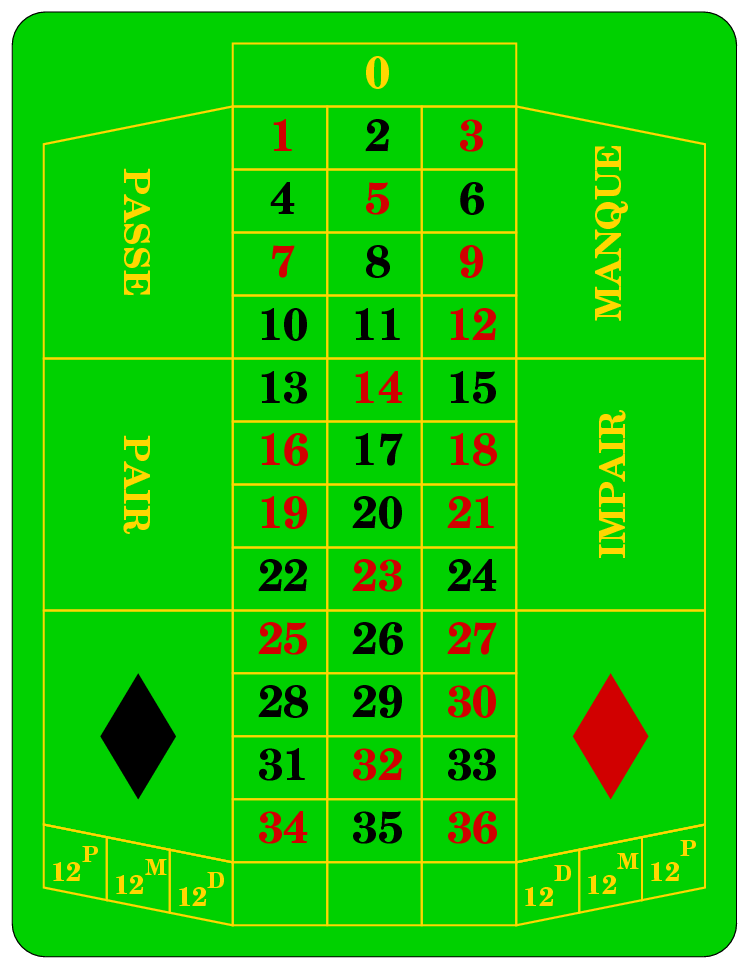
\includegraphics[height=10truecm]{graphics/Roulette_frz}
\end{center}
\caption{Spielfeld des franz"osischen Roulette\label{roulette-feld}}
\end{figure}
Die Roulettespieler setzen Chips auf das Spielfeld gem"ass Abbildung~\ref{roulette-feld}, welches ausser Feldern
f"ur die Zahlen 0 bis 36 auch Felder enth"alt, welche f"ur Teilmengen
von Zahlen stehen. So stehen ``pair'' und ``impair'' f"ur die 18 geraden
bzw.~ungeraden Zahlen, ``rouge'' und ``noir'' f"ur die rot bzw.~schwarz
eingef"arbten Zahlen und ``passe'' und ``manque'' f"ur die obere bzw.~untere
H"alfte der Zahlen. Wichtig ist dabei, dass diese Sammelfelder die
Null niemals umfassen. Man kann auch auf die Zahlen setzen die bei Teilung
durch $3$ den Rest $1$, $2$ oder $0$ ergeben, dazu dienen die leeren
Felder am der Null gegen"uberliegenden Ende des Zahlenfeldes.
Die mit $\mathstrut^D12$, $\mathstrut^M12$ und $\mathstrut^P12$
bezeichneten Felder stehen jeweils f"ur das untere, mittlere und obere
Drittel der Zahlen. Chips d"urfen auch auf Begrenzungslinien zwischen zwei
Feldern gesetzt werden, oder auf Schnittpunkte.
Ein Chip auf dem Schnittpunkt, der den Feldern $4$, $5$, $7$ und $8$
gemeinsam ist, bedeutet einen Einsatz von je einem Viertel des
Chipwertes auf jede der vier Zahlen.

Die Eins"atze m"ussen gespielt werden, w"ahrend
\index{Croupier}
des Rouletterad sich dreht. Sobald der Croupier ``rien ne va plus'' ruft,
darf nicht mehr gesetzt werden. Es gewinnt jene Zahl, in deren Fach
im Rouletterad die Kugel f"allt.

Der Gewinn wird wie folgt ausbezahlt. Steht ein Feld f"ur eine einzige
Zahl, dann wird das sechsundreissigfache des Einsatzes ausbezahlt.
Steht ein Feld f"ur $n$ Zahlen aus der Menge $\{1,\dots,36\}$, dann
reduziert sich der Gewinn um den Faktor $n$. Zeigt das Rouletterad
die Zahl $1$, dann gewinnen Chips auf ``rouge'', ``impair'' und ``manque''
je das doppelte des Einsatzes. Ein Chip auf $\mathstrut^M 12$ dagegen
gewinnt das dreifache des Einsatzes, dieses Feld steht f"ur $n=12$.
Setzt ein Spieler einen Chip auf die Linie zwischen den Zahlen $1$ und
$2$, und wird zwei gezeigt, dann gewinnt er das 18-fache des Einsatzes,
denn die Linie steht f"ur eine Menge von $n=2$ Zahlen.

Die Null hat eine besondere Bedeutung. Zeigt das Rouletterad die
Null, gewinnen einzig und allein die Chips, die auf 0 gesetzt wurden,
und zwar das 36-fache des Einsatzes.

\subsection{Gewinnwahrscheinlichkeiten}
\index{Roulette!Gewinnwahrscheinlichkeit}
Offenbar ist es eine vern"unftige Annahmen, jede der 37 Zahlen $0,\dots,36$
f"ur gleich wahrscheinlich anzusehen. Ein ideales, faires Rouletterad
wird jede dieser Zahlen etwa gleich h"aufig zeigen. Die Wahrscheinlichkeit
f"ur das Ereignis
$\omega_x=\{\text{das Rouletterad zeigt die Zahl $x$}\}$
ist daher 
$P(\omega_x)=\frac{1}{37}.$
Diese Ereignisse schliessen sich offensichtlich gegenseitig aus:
$\omega_x\cap\omega_y=\emptyset$ falls $x\ne y$. Damit l"asst sich auch
die Wahrscheinlichkeit daf"ur berechnen, dass das Rouletterad eine
Zahl aus einer Teilmenge $A\subset\{0,\dots,36\}$ zeigt. Das entsprechende
Ereignis ist $\omega_A=\bigcup_{x\in A}\omega_x$,
und seine Wahrscheinlichkeit ist
\[
P(\omega_A)=P(\bigcup_{x\in A}\omega_x)=\sum_{x\in A}P(\omega_x)=|A|\frac1{37}.
\]

Der Einsatz auf einem Feld, welches f"ur die Menge $A$ steht, ergibt
einen Gewinn von $\frac{36}{|A|}$, und folglich ist der bei h"aufiger
Wiederholung des gleichen Einsatzes "uber lange Zeit zu erwartende Gewinn
pro Chip
\[
\frac{36}{|A|}\cdot P(\omega_A)=\frac{36}{37}=0.\overline{972}<1.
\]
Insbesondere kann man langfristig nicht damit rechnen, den ganzen
Einsatz je wieder zur"uckzuerhalten, ein 37stel ($2.7\%$) des Einsatzes gehen
im Mittel an das Casino.

Offensichtlich ist das Vorhandensein der Zahl $0$ f"ur das Casino
ein Segen. G"abe es die Null nicht, w"are die Wahrscheinlichkeit
der Ereignisse $\omega_x$ jeweils $P(\omega_x)=\frac1{36}$, und
der langfristig zu erwartende Gewinn pro Einsatz w"are $\frac{36}{36}=1$.
Damit w"urde es f"ur eine Casino jedoch schwierig, einen zuverl"assigen
Gewinn zu realisieren, und auch die oben erw"ahnten $2.7\%$ sind manchem
Casino-Betreiber zu wenig. Mit einem zus"atzlichen m"oglichen Ausgang
des Rouletterades, der Doppelnull, die bei der Gewinnauszahlung
genau wie die einfache Null behandelt wird, steigt der durchschnittlich
an das Casino fliessende Betrag auf $5.26\%$. Somit kostet ein Einsatz
in so einem Casino mehr als im Moment in der Schweiz eine Hypothek. Wenn
man also Geld braucht, nimmt man es besser bei der Bank auf, als dass man
in einem Casino auf einen Gewinn hoft.

\subsection{Gibt es eine Gewinnstrategie f"ur Roulette?}
\index{Roulette!Gewinnstrategie}
Die Berechnungen des voranstehenden Abschnittes beweisen noch nicht,
dass es keine Strategie gibt, mit der man im Roulette trotzdem
gewinnen k"onnte.
%Wir werden auf diese Frage in Abschnitt
%\ref{roulette-strategie}
%zur"uckkommen.

Es gibt jedoch auch ein weniger mathematisches Argument, welches
die Existenz einer Gewinnstrategie unwahrscheinlich erscheinen l"asst.
Spiel-Casinos sind keine sozialen Institutionen, die dazu da sind,
ihre Kundschaft zu bereichern. Ganz im Gegenteil.
Sie sind Wirtschaftsunternehmen, welche wie andere Unternehmen auch
L"ohne und Steuern bezahlen m"ussen, f"ur ihre Lokale Mieten zahlen 
und f"ur ihren Energieverbrauch und f"ur Telekommunikationsverbindungen
Geb"uhren zahlen m"ussen. Ausserdem erwarten die Investoren, dass
sie einen Gewinn erwirtschaften, und eine m"oglichst attraktive
Dividende aussch"utten. Und die Spieler erwarten nat"urlich auch,
dass die erspielten Gewinne ausbezahlt werden.
All diesen Ausgaben stehen als einzige
Einnahmequelle die Eins"atze der Spieler gegen"uber\dots

\section{Anzahl eingetroffene Ereignisse}
Wir betrachten ein Experiment mit zwei m"oglichen Ausg"angen, die
wir postiv bzw.~negativ nennen. Die Wahrscheinlichkeit dieser beiden
Ausg"ange ist $p$ bzw.~$1-p$.
Wiederholt man das Experiment mit zwei m"oglichen Ausg"angen mit
Wahrscheinlichkeiten $p$ und $1-p$ $n$ mal, kann man nach der Anzahl 
der ``erfolgreichen'' Ausg"ange des Experiments fragen. Damit wird
ein neues Ereignis definiert: 
\[
A_k=\{\text{Anzahl positiver Ausg"ange ist $k$}\}
\]
Und wir k"onnen nach der Wahrscheinlichkeit $P(A_k)$ fragen.
Die Wahrscheinlichkeit einer ganz bestimmten Abfolge von positiven
und negativen Ausg"angen ist 
\[
P(\text{\tt ++-+-++--+})=
P(\text{\tt +})
P(\text{\tt +})
P(\text{\tt -})
P(\text{\tt +})
P(\text{\tt -})
P(\text{\tt +})
P(\text{\tt +})
P(\text{\tt -})
P(\text{\tt -})
P(\text{\tt +})
=p^6(1-p)^4
\]
In diesem Beispiel waren sechs Ausg"ange positiv, allgemein ist die
Wahrscheinlichkeit einer ganz bestimmten Abfolge enthaltend $k$ positive
Ausg"ange $p^k(1-p)^{n-k}$.

Nun gibt es aber verschiedene M"oglichkeiten, wie die {\tt +}
und {\tt -} angeordnet sein k"onnen. Insgesamt gibt es 
$\binom{n}k$ Arten, wie die $k$ positiven Ausg"ange platziert sein
k"onnen, also ist die Wahrscheinlichkeit
\[
P(A_k)=
\binom{n}{k}p^k(1-p)^{n-k}.
\]
Damit l"asst sich jetzt auch die Wahrscheinlichkeit berechnen, dass die
Anzahl $k$ in einem bestimmten Intervall liegt:
\[
P(a \le k\le b)
=
\sum_{k=a}^b \binom{n}{k}p^k(1-p)^{n-k}.
\]
Das Intervall $0\le k\le n$ umfasst alle m"oglichen F"alle, und sollte
daher die Wahrscheinlichkeit $1$ ergeben:
\[
P(0\le k\le n)=
\sum_{k=0}^n \binom{n}{k}p^k(1-p)^{n-k}=
(p+(1-p))^n=1^n=1.
\]



